\documentclass[14pt, a4paper]{article}

\usepackage{amssymb}
\usepackage{extsizes}
\usepackage{graphicx}
\usepackage{xcolor}
\usepackage{caption}
\usepackage{listings}
\usepackage{tabularx}
\usepackage{indentfirst}
\usepackage[T2A]{fontenc}
\usepackage[utf8]{inputenc}
\usepackage[english,russian]{babel}
\usepackage[left=30mm, right=10mm, top=20mm, bottom=20mm]{geometry}
\usepackage{ucs}

\graphicspath{{images/}}

\linespread{1.3}
\setcounter{tocdepth}{4}
\setlength{\parskip}{1.5pt}

\begin{document}
	\section*{Продолжение}
	
	О модели <<многие-ко-многим>> можно сказать, что пользователь не имеет ограничений на количество создаваемых потомков, при этом потомки, созданные в пространтсве пользователя, соответствуют потокам ядра. Таким образом, блокировка одного потока не приводит к блокировке остальных.
	
	!!! Реальное распараллеливание возможно на реальных процессорах (речь идет о распараллеливании по данным).
	
	Распараллеливание по функции совсем другое. Ярчайший пример - текстовый редактор (по задачам, которые стоят перед редактором). Самое важное - выделить в отдельный поток ввод/вывод, так как ввод/вывод связан с блокировкой (если это возможно).
	
	Даже если у нас один единственный процессор, то все равно в многозадачных системах разделения времени процессы выполняются квазипараллельно (с точки зрения команд - последовательно, а с точки зрения пользователя - параллельно, так как пользователю важна отзывчивость системы).
	
	Почему в однопроцессорной машине нужно использовать многопоточность? Потому что в системе самым медленным звеном является человек. То есть количество потоков, которые может запустить пользователь, - это его произвол. Это наше решение, но оно должно быть обоснованным, и не последнюю роль играет в этом аппаратная часть
	
	\subsection*{Двухуровневая модель}
	
	[картинка]
	
	Для общности управления выполнением работы в системе разведены в потоки, если не создаем в системе ни одного потока, то считается в системе, что создан один главный поток.
	
	\subsection*{Библиотеки потоков}
	
	Потоки бывают уровня пользователя и уровня ядра, но есть смешанная модель. Пример: В системе Solaris глубоко проработан вопрос потоков. Сначала появились потоки уровня пользователя [...].
	
	В настоящее время поддерживаются потоки уровня ядра. Должны быть соотвтетствующие библиотеки. Существуют три основные билиотеки потоков.
	
	\begin{enumerate}
		\item POSIX Pthreads
		
		POSIX (Portable Operating System Interface for UNIX) - это стандарт/спецификация, <<предназначенная для правительственных учреждений, покупающих ПО>>. Регламентирует системные вызовы, обрабатываемые системой, чтобы ПО было переносимо. Определяет потоки и уровня пользователя, и уровня ядра.
		
		\item Win32 threads
		
		Библиотека уровня ядра (винда)
		
		\item Java threads
		
		Когда говорят о программе на джаве, то говорят на джава-виртуальной машине.
		
		!!! Потоки увеличивают объем памяти под кучи (???)
		
		<<Потоки - это совсем не безобидная игрушка>>
	\end{enumerate}

	{\it Про джаву: Все джава программы используют потоки, даже обычная однопоточная программа. JVM - основная часть исполняющей системы джавы, и в ней создание новых потоков требует [чего-то там]. При этом любой потомок класса thread содержит public void run.}
	
	OpenMP - набор директив компилятора, допустимые для C/C++ (и даже для Fortran). В результате, компилятор автоматически сгенерирует параллельное выполнение.

	\begin{lstlisting}
#pragma omp parallel
{
	/* some parallel code */
}
	\end{lstlisting}

	\section*{Диаграмма состояния процесса в UNIX}
	
	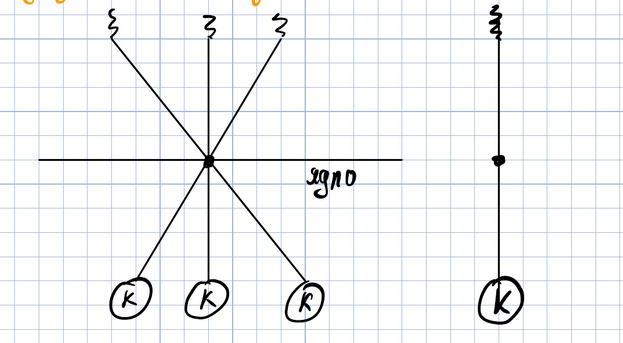
\includegraphics[width=\linewidth]{2}
	
	{\it Между выполнением в режиме ядра и прекращением существования нужно нарисовать состояние Зомби}
	
	Важно понимать, что все эти действия выполняются в режиме ядра, за исклчением выполнения кода приложения.
	
	В первом классическом UNIX использовалась память сегментами по запросу.
	
	\section*{Взаимодествие параллельных процессов}
	
	Речь идет о любой параллельности.
	
	Проблема: Рассмотрим пример
	
	\begin{lstlisting}
P1:
	mov eax, myvar
	inc eax
	mov myvar eax

P2:
	mov eax, myvar
	inc eax
	mov myvar, eax
	\end{lstlisting}

	\begin{itemize}
		\item Реальная параллельность
		
		[таблица 1]
		
		\item Квазипараллельность
		
		[таблица 2]
	\end{itemize}

	[потоки переменные, критическая область программы CR (обычная - PR)]
	
	Для решения проблемы необходимо обеспечить монопольный доступ процессов к критической секции (к разделяемым переменным). Это значит, что только один процесс должен получать доступ к критической секции. Это обеспечивается методами взаимоисключения: если один процесс находится в критической секции, то другой не может войти в эту же критическую секцию.
	
	Монопольный доступ обсепечивается следующими методами/способами:
	
	\begin{itemize}
		\item программным
		\item аппаратным
		\item с помощью семафоров
		\item с помощью мониторов
	\end{itemize}

	Системы и их ПО не стоит на месте, так что имеются и другие средства.
	
	\subsection*{Программные методы взаимоскючения}
	
	Идея: использовать флаг
	
	Псевдокод
	
	\begin{lstlisting}
program exmp1;

flag1, flag2: logical;
flag1 = 0; flag2 = 0;

p1: while(1) do;
	while(flag2) do;
	flag1 = 1;
	CR1;
	flag1 = 0;
	PR1;
	end;

p2: while(1) do;
	while(flag2) do;
	flag2 = 1;
	CR2;
	flag2 = 0;
	PR2;
	end;

parbegin:
	p1; p2;
parend;

end;
	\end{lstlisting}

	[анализ]
	
	Следовательно, данный способ не реализует монопольный доступ.
	
	Другой вариант - установить флаг до проверки условия цикла.
	
	\begin{lstlisting}
program exmp2;

flag1, flag2: logical;

flag1 = 0; flag2 = 0;

p1: while(1) do;
	flag1 = 1;
	while(flag2) do;
	CR1;
	flag1 = 0;
	PR1;
	end;

p2: while(1) do;
	flag2 = 1;
	while(flag1) do;
	CR2;
	flag2 = 0;
	PR2;
	end;

parbegin:
	p1; p2;
parend;

end;	
	\end{lstlisting}
	
	Пусть инициатива у P2. Он сразу устанавливает флаг и теряет флаг до проверки. P1 устанавливает фла и заходит в цикл проверки... Исчерпывает квант. Получается, что P1 и P2 ждут завершения друг друга и зависают (dead lock).
	
	В итоге, решение тоже не рабочее.
	
	Dekker предложил решение задачи (корректное), но только для двух процессов. Он ввел дополнительную переменную, которая определяется, как переменная-очередь.
	
	\begin{lstlisting}
program exmp3;

f1, f2: logical;
que: int;

p1: while(1) do
	begin
		f1 = true;
		while(f2 == 1) do
		begin
			if(que == 2) then
			begin 
				f1 = false;
				while (que == 2) do;
				f1 = true;
			end;
			CR1;
			f1 = false;
			que = 2;
			PR1;
		end;
	end;

p2: ...
	\end{lstlisting}
\end{document}
